\begin{frame}

Part 1:
\vspace{0.2cm}

{\LARGE \textbf{\textcolor{blue}{Abstract Domain}}}

\end{frame}




\begin{frame}[fragile]{\textcolor{blue}{Background to LLVM Integer Types}}
\begin{itemize}
\item In LLVM the type of $N$-bit integers is the set $\texttt{i}N \coloneqq \{0,1\}^N, \text{for~} N \in \{1,\dots, 2^{23}-1\}$.
\item "$\texttt{i}N \cong \mathbb{Z}/2^N$~"
\item In the in-memory-representation, these types are represented by the LLVM class APInt.
\item This type is used for both signed and unsigned integers.

\item We use APInt 	 in our implementation of abstract domains.

\end{itemize}

\end{frame}

\begin{frame}[fragile]{\textcolor{blue}{LLVM Integer Operations}}
\begin{large}Arithmetic Operations:\end{large} \\
In LLVM there are separate $\texttt{div}$ and $\texttt{rem}$ operations for signed and unsigned integers.
For $\texttt{add}$, $\texttt{sub}$ and $\texttt{mul}$, there is no such distinction needed.
\begin{itemize}
\item $\texttt{<result> = add [nuw] [nsw] <bitWidth> <op1> <op2>}$
\item $\texttt{<result> = sub [nuw] [nsw] <bitWidth> <op1> <op2>}$
\item $\texttt{<result> = mul [nuw] [nsw] <bitWidth> <op1> <op2>}$
\item $\texttt{<result> = udiv [exact] <bitWidth> <op1> <op2>}$
\footnote{\label{not-impl} $\texttt{exact}$-flag not used in our implementation.}
\item $\texttt{<result> = sdiv [exact] <bitWidth> <op1> <op2>} ^{~\ref{not-impl}}$
\item $\texttt{<result> = urem <bitWidth> <op1> <op2>}$
\item $\texttt{<result> = srem <bitWidth> <op1> <op2>}$
\end{itemize}

$\texttt{nuw}$ : "no unsigned wrap", $\texttt{nsw}$ : "no signed wrap"

\end{frame}

\begin{frame}[fragile]{\textcolor{blue}{LLVM Integer Operations (cont.)}}
Bitwise Operations:
\begin{itemize}
\item $\texttt{<result> = shl [nuw] [nsw] <bitWidth> <op1> <op2>}$
\item $\texttt{<result> = lshr [exact] <bitWidth> <op1> <op2>}$ \footnote{\label{not-impl2} $\texttt{exact}$-flag not used in our implementation.}
\item $\texttt{<result> = ashr [exact] <bitWidth> <op1> <op2>}^{~\ref{not-impl2}}$
\item $\texttt{<result> = and <bitWidth> <op1> <op2>}$
\item $\texttt{<result> = or <bitWidth> <op1> <op2>}$
\item $\texttt{<result> = xor <bitWidth> <op1> <op2>}$
\end{itemize}

\end{frame}

\begin{frame}[fragile]{\textcolor{blue}{Bounded Set}}
\begin{itemize}
\item A bounded set represents a set of values up to a given cardinality $k$, or $\top$: \\
$\mathrm{BS}_{N} \coloneqq \{M\in \mathcal{P}(\texttt{i}N)\mid |M| \leq k\} \dot\cup \{ \top \}$ \\
\item $\sqcup$ and $\sqsubseteq$ on bounded sets essentially reduce to $\cup$ and $\subseteq$ on sets.
\item Any set with more elements than $k$ is over-approximated by $\top$.
\item $\gamma_{BS_N} \colon \mathrm{BS}_N \rightarrow \mathcal{P}(\texttt{i}N),
b \mapsto
\begin{cases}
\texttt{i}N,  & \text{if }b=\top \\
b, & \text{otherwise}
\end{cases}
$

\end{itemize}

\end{frame}


\begin{frame}[fragile]{\textcolor{blue}{Modular Strided Interval (MSI)}}
\begin{itemize}

\item Intervals:
\begin{itemize}
\item $\mathsf{I} \coloneqq [a,b], \text{for } a,b \in \mathbb{Z}$
\end{itemize}
\item Strided Intervals:
\begin{itemize}
\item $\mathsf{SI} \coloneqq s[a,b], \text{for } a,b \in \mathbb{Z}, s \in \mathbb{N}$
\item $\gamma_{\mathsf{SI}} \colon \textsf{SI}_N \rightarrow \mathcal{P}(\mathbb{Z}), s[a,b] \mapsto \{k \in \mathbb{Z} \mid
a \leq k \leq b, k \equiv a \mod s \}$
\end{itemize}
\item Modular Strided Intervals:
\begin{itemize}
\item $\mathsf{MSI}_{N} \coloneqq \{s[\overline{a},\overline{b}]_N \mid \overline{a}, \overline{b} \in \mathbb{Z}/2^N, s \in \{0, \dots, 2^N\} \}\;\dot\cup\;\{\bot\}$
\item {\setlength{\abovedisplayskip}{-10pt}\begin{flalign*}
\gamma_{\mathsf{MSI}_N} \colon & \textsf{MSI}_N \rightarrow \mathcal{P}(\texttt{i}N), \\
& i \mapsto \begin{cases}
\emptyset, & \text{if }i = \bot \\
\parbox[t]{.53\textwidth}{$\{k + 2^N\mathbb{Z} \mid
k \in \mathbb{Z}, a \leq k \leq c, k \equiv a \mod s \}$, \\
$\text{\quad where }c = \min\{x \in \mathbb{Z} \mid x \geq a,$ \\
$\text{\quad\quad} x \equiv b \mod 2^N \}$}, & \text{if }i = s[\overline{a},\overline{b}]_N
\end{cases}
\end{flalign*}}
\item Examples:
\begin{itemize}
\item $12[15,63]_8 \stackrel{\gamma\;}{\rightarrow}\{15,27,39,51,63\} \subseteq \mathbb{Z}/2^8$
\item $4[10,6]_4 \stackrel{\gamma\;}{\rightarrow}\{10,14,2,6\} \subseteq \mathbb{Z}/2^4$

\end{itemize}
\end{itemize}
\end{itemize}

\end{frame}


\begin{frame}[fragile]{\textcolor{blue}{Modular Strided Interval: Normalization}}
Note that some sets can be represented by muliple MSIs. Thus, we introduce a predicate \textit{normal}, such that there is at most one \textit{normalized} representation.
Examples: \\
\def\arraystretch{6}
\begin{tabular}{ l l l l }
\adjustbox{valign=c}{\parbox[t]{1.25cm}{\centering
$3[2, 10]_4$ \\
$\downarrow$ \\
$3[2, 8]_4$}} &
\begin{minipage}{0.3\textwidth}
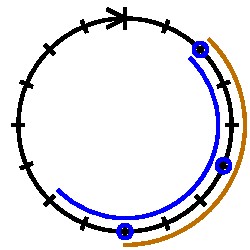
\includegraphics[width=0.75\textwidth]{graphics/msi-normalization-1.pdf}
\end{minipage}
\adjustbox{valign=c}{\parbox[t]{1.25cm}{\centering
$4[3, 3]_4$ \\
$\downarrow$ \\
$0[3, 3]_4$}} &
\begin{minipage}{0.3\textwidth}
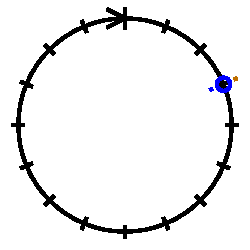
\includegraphics[width=0.75\textwidth]{graphics/msi-normalization-2.pdf}
\end{minipage} \\
\adjustbox{valign=c}{\parbox[t]{1.25cm}{\centering
$6[12, 2]_4$ \\
$\downarrow$ \\
$10[2, 12]_4$}} &
\begin{minipage}{0.3\textwidth}
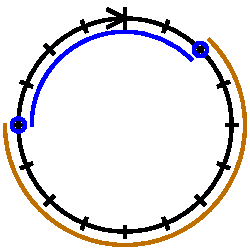
\includegraphics[width=0.75\textwidth]{graphics/msi-normalization-3.pdf}
\end{minipage}
\adjustbox{valign=c}{\parbox[t]{1.25cm}{\centering
$4[10, 6]_4$ \\
$\downarrow$ \\
$4[2, 14]_4$}} &
\begin{minipage}{0.3\textwidth}
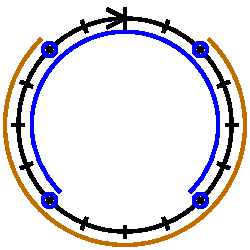
\includegraphics[width=0.75\textwidth]{graphics/msi-normalization-4.pdf}
\end{minipage}
\end{tabular}
\end{frame}


\begin{frame}[fragile]{\textcolor{blue}{Modular Strided Interval: Normalization (cont.)}}
\begin{flalign*}
& \rlap{\(\mathsf{normal}_N(s[\overline{a}, \overline{b}]_N) \leftrightarrow (\)} &
\end{flalign*}
{\setlength{\abovedisplayskip}{-6pt}\begin{flalign*}
\quad & \overline{a} = \overline{b} \rightarrow s = 0 & \\
\quad \land\ & \overline{b} \in \gamma_N(s[\overline{a}, \overline{b}]_N) & \\
\quad \land\; & \overline{a} = \min\{a' \in \{0 \ldots 2^N-1\} \ldotp \exists s', \overline{b}' \ldotp \gamma_N(s'[\overline{a'}, \overline{b}']_N) = \gamma_N(s[\overline{a}, \overline{b}]_N)\} + 2^N \mathbb{Z} &
\end{flalign*}}
{\setlength{\abovedisplayskip}{-18pt}\begin{flalign*}
& ) &
\end{flalign*}}
\end{frame}

\begin{frame}[fragile]{\textcolor{blue}{Modular Strided Interval: Union}}
MSIs do not form a lattice, as, in general, there is no \textit{least} upper bound of two elements. \\
Example:
\begin{tabular}{ l l l l l }
\adjustbox{valign=c}{\parbox[t]{1.25cm}{\centering
$1[1, 5]_4$}} &
\begin{minipage}{0.3\textwidth}
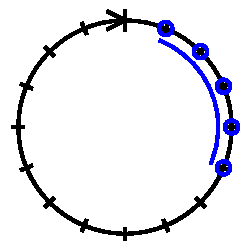
\includegraphics[width=0.75\textwidth]{graphics/msi-union-1.pdf}
\end{minipage} & $\sqcup$ &
\adjustbox{valign=c}{\parbox[t]{1.25cm}{\centering
$1[9, 12]_4$}} &
\begin{minipage}{0.3\textwidth}
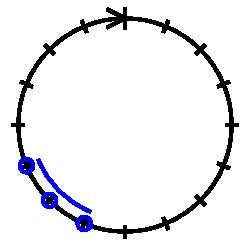
\includegraphics[width=0.75\textwidth]{graphics/msi-union-2.pdf}
\end{minipage} \\
&& $=$ && \\
\adjustbox{valign=c}{\parbox[t]{1.25cm}{\centering
$1[1, 12]_4$}} &
\begin{minipage}{0.3\textwidth}
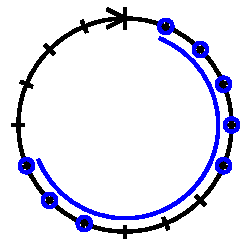
\includegraphics[width=0.75\textwidth]{graphics/msi-union-3.pdf}
\end{minipage} & or &
\adjustbox{valign=c}{\parbox[t]{1.25cm}{\centering
$1[9, 5]_4$}} &
\begin{minipage}{0.3\textwidth}
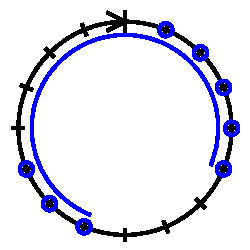
\includegraphics[width=0.75\textwidth]{graphics/msi-union-4.pdf}
\end{minipage}
\end{tabular} \\
Therefore we try to find a \textit{minimal} upper bound wrt. $|\gamma(\cdot)|$.
\end{frame}


\begin{frame}[fragile]{\textcolor{blue}{Abstract Domain Class Structure}}

\begin{center}
\begin{tikzpicture}[thick,scale=0.8, every node/.style={transform shape}]

\umlinterface[]{AbstractDomain}{
}{
add(other) : AbstractDomain \\ /* other arithmetic and logical operations */ \\ \\

icmp(other, predicate) : (AbstractDomain, AbstractDomain) \\ \\
leastUpperBound(other) : AbstractDomain \\
lessOrEqual(other) : bool \\
}

\umlclass[x=-3.5,y=-4.0]{CompositeDomain}{delegate : AbstractDomain}{}
\umlclass[x=+3.0,y=-3.9]{BoundedSet}{
values : set$<$APInt$>$ \\
isTop : bool}{}
\umlclass[x=+3.0,y=-6.3]{StridedInterval}{
min, max, stride : APInt \\
isBottom : bool}{}


%\umlclass[x=-3,y=-6.5]{OperationNDim$<$vec$>$}{}{}

%\umlclass[x=3,y=-6.5]{OperationNDim$<$novec$>$}{}{}

\umlimpl[anchor1=north,anchor2=-148]{CompositeDomain}{AbstractDomain}
\umlimpl[anchor1=north,anchor2=-36]{BoundedSet}{AbstractDomain}
\umlimpl[geometry=-|-, arm1=0.5cm,anchors=east and east]{StridedInterval}{AbstractDomain}
%\umlaggreg[]{OperationNDim$<$T;U;V$>$}{OperationMass}
%\umlaggreg[]{OperationNDim$<$T;U;V$>$}{OperationConvection}
\umlaggreg[]{CompositeDomain}{BoundedSet}
\umlaggreg[geometry=-|-,anchors=east and west]{CompositeDomain}{StridedInterval}


\end{tikzpicture}
\end{center}

\end{frame}

\begin{frame}[fragile]{\textcolor{blue}{Application Interface}}

\begin{minipage}{0.5\textwidth}
\begin{center}
\begin{tikzpicture}[thick,scale=0.8, every node/.style={transform shape}]

\umlclass[fill=red!20,y=+5, x=-6.5
]{VSAResult}{}{
is\_reachable(basic\_block) : bool \\
is\_resultat\_available(bb, value) : bool \\
get\_abstract\_value() : VSAResultValue \\
}

\umlclass[fill=red!20,y=1.5, x=-6.5]{VSAResultValue}{
}{
test(predicate, constant) : tristate \\
min() : APInt \\
max() : APInt \\
size() : APInt \\
constant() : APInt \\
is\_constant() : bool \\
}

\end{tikzpicture}
\end{center}
\end{minipage}
\begin{minipage}{0.49\textwidth}
\begin{itemize}
\item after a successful pass:\\
\quad {\color{blue} auto\& res = vsap.get\_result();}
\item query information related to \\basic block (reachable or not) and/or variable (abstract value)\\
%\quad {\color{blue} auto\& res = vsap.get\_result();}
\end{itemize}
\end{minipage}

\end{frame}

\begin{frame}[fragile]{\textcolor{blue}{Connection of the Results to the Internal Abstract Domain}}

\begin{center}
\begin{tikzpicture}[thick,scale=0.8, every node/.style={transform shape}]

\umlinterface[rectangle split parts=1, x=1.0, y=-1.0]{AbstractDomain}{
}{}

\umlclass[x=-3.5,y=-3.5, rectangle split parts=1]{CompositeDomain}{}{}
\umlclass[x=+1.0,y=-3.5, rectangle split parts=1]{BoundedSet}{}{}
\umlclass[x=+2.0,y=-5.5, rectangle split parts=1]{StridedInterval}{}{}

\umlclass[fill=red!20
%,y=+3
,y=0.5, x=-6.5
]{VSAResultValue}{
}{
test(predicate, constant) : tristate \\
min() : APInt \\
max() : APInt \\
size() : APInt \\
constant() : APInt \\
is\_constant() : bool \\
}

%\umlclass[x=-3,y=-6.5]{OperationNDim$<$vec$>$}{}{}

%\umlclass[x=3,y=-6.5]{OperationNDim$<$novec$>$}{}{}

\umlimpl[geometry=|-]{CompositeDomain}{AbstractDomain}
\umlimpl[anchor1=north,anchor2=south]{BoundedSet}{AbstractDomain}
\umlimpl[geometry=-|-, arm1=0.5cm,anchors=east and east]{StridedInterval}{AbstractDomain}
%\umlaggreg[]{OperationNDim$<$T;U;V$>$}{OperationMass}
%\umlaggreg[]{OperationNDim$<$T;U;V$>$}{OperationConvection}
\umlaggreg[]{CompositeDomain}{BoundedSet}
\umlaggreg[geometry=-|-,anchors=east and west]{CompositeDomain}{StridedInterval}

\umlaggreg[geometry=|-|,anchor1=north,anchor2=north,arm1=0.5cm]{VSAResultValue}{AbstractDomain}

\end{tikzpicture}
\end{center}

\end{frame}
